\subsection{Простое шифрование используя XOR-маску}
\label{XOR_mask_1}

Я нашел одну старую игру в стиле interactive fiction в архиве \IT{if-archive}\footnote{\url{http://www.ifarchive.org/}}:

\begin{lstlisting}
The New Castle v3.5 - Text/Adventure Game
in the style of the original Infocom (tm)
type games, Zork, Collosal Cave (Adventure),
etc.  Can you solve the mystery of the
abandoned castle?
Shareware from Software Customization.
Software Customization [ASP] Version 3.5 Feb. 2000
\end{lstlisting}

Можно скачать здесь: \url{https://github.com/DennisYurichev/RE-for-beginners/blob/master/ff/XOR/mask_1/files/newcastle.tgz}.

Там внутри есть файл (с названием \IT{castle.dbf}), который явно зашифрован, но не настоящим криптоалгоритмом,
и оне сжат, это что-то куда проще.
Я бы даже не стал измерять уровень энтропии (\myref{entropy}) этого файла, потому что я итак уверен, что он низкий.
Вот как он выглядит в Midnight Commander:

\begin{figure}[H]
\centering
\myincludegraphics{ff/XOR/mask_1/mc_encrypted.png}
\caption{Зашифрованный файл в Midnight Commander}
\end{figure}

Зашифрованный файл можно скачать здесь:
\url{https://github.com/DennisYurichev/RE-for-beginners/blob/master/ff/XOR/mask_1/files/castle.dbf.bz2}.

Можно ли расшифровать его без доступа к программе, используя просто этот файл?

Тут явно просматривается повторяющаяся строка. 
Если использовалось простое шифрование с XOR-маской, такие повторяющиеся строки это явное свидетельство,
потому что, вероятно, тут были длинные лакуны с нулевыми байтами, которые, в свою очередь, присутствуют
во мноигих исполняемых файлах, и в остальных бинарных файлах.

\myindex{UNIX!xxd}
Вот дам начала этого файла используя утилиту \IT{xxd} из UNIX:

\lstinputlisting{ff/XOR/mask_1/xxd_result.txt}

Давайте держаться за повторяющуюся строку \TT{iubgv}.
Глядя на этот дамп, мы можем легко увидеть, что период повторений этой строки это 0x51 или 81.
Вероятно, 81 это длина блока?
Длина файла 1658961, и она может быть поделена на 81 без остатка (и тогда там 20481 блоков).

Теперь я буду использовать Mathematica для анализа, есть ли тут повторяющиеся 81-байтные блоки в файле?
Я разделю входной файл на 81-байтные блоки и затем использую ф-цию
\IT{Tally[]}\footnote{\url{https://reference.wolfram.com/language/ref/Tally.html}}
которая просто считает, сколько раз каждый элемент встретился во входном списке.
Вывод Tally не отсортирован, так что я также добавлю ф-цию \IT{Sort[]} для сортировки его по кол-ву вхождений
в нисходящем порядке.

\begin{lstlisting}[style=custommath]
input = BinaryReadList["/home/dennis/.../castle.dbf"];

blocks = Partition[input, 81];

stat = Sort[Tally[blocks], #1[[2]] > #2[[2]] &]
\end{lstlisting}

И вот вывод:

\begin{lstlisting}[style=custommath]
{{{80, 103, 2, 116, 113, 102, 118, 25, 99, 8, 19, 23, 116, 125, 107, 
   25, 99, 109, 114, 102, 14, 121, 115, 31, 9, 117, 113, 111, 5, 4, 
   127, 28, 122, 101, 8, 110, 14, 18, 124, 106, 16, 20, 104, 119, 8, 
   109, 26, 106, 9, 97, 13, 99, 15, 119, 20, 105, 117, 98, 103, 118, 
   1, 126, 29, 97, 122, 17, 15, 114, 110, 3, 5, 125, 125, 99, 126, 
   119, 102, 30, 122, 2, 117}, 1739}, 
{{80, 100, 2, 116, 113, 102, 118, 25, 99, 8, 19, 23, 116, 
   125, 107, 25, 99, 109, 114, 102, 14, 121, 115, 31, 9, 117, 113, 
   111, 5, 4, 127, 28, 122, 101, 8, 110, 14, 18, 124, 106, 16, 20, 
   104, 119, 8, 109, 26, 106, 9, 97, 13, 99, 15, 119, 20, 105, 117, 
   98, 103, 118, 1, 126, 29, 97, 122, 17, 15, 114, 110, 3, 5, 125, 
   125, 99, 126, 119, 102, 30, 122, 2, 117}, 1422}, 
{{80, 101, 2, 116, 113, 102, 118, 25, 99, 8, 19, 23, 116, 
   125, 107, 25, 99, 109, 114, 102, 14, 121, 115, 31, 9, 117, 113, 
   111, 5, 4, 127, 28, 122, 101, 8, 110, 14, 18, 124, 106, 16, 20, 
   104, 119, 8, 109, 26, 106, 9, 97, 13, 99, 15, 119, 20, 105, 117, 
   98, 103, 118, 1, 126, 29, 97, 122, 17, 15, 114, 110, 3, 5, 125, 
   125, 99, 126, 119, 102, 30, 122, 2, 117}, 1012},
{{80, 120, 2, 116, 113, 102, 118, 25, 99, 8, 19, 23, 116, 
   125, 107, 25, 99, 109, 114, 102, 14, 121, 115, 31, 9, 117, 113, 
   111, 5, 4, 127, 28, 122, 101, 8, 110, 14, 18, 124, 106, 16, 20, 
   104, 119, 8, 109, 26, 106, 9, 97, 13, 99, 15, 119, 20, 105, 117, 
   98, 103, 118, 1, 126, 29, 97, 122, 17, 15, 114, 110, 3, 5, 125, 
   125, 99, 126, 119, 102, 30, 122, 2, 117}, 377},

...

{{80, 2, 74, 49, 113, 21, 62, 88, 39, 71, 68, 23, 63, 51, 36, 78, 48, 
   108, 114, 102, 14, 121, 115, 31, 9, 117, 113, 111, 5, 4, 127, 28, 
   122, 101, 8, 110, 14, 18, 124, 106, 16, 20, 104, 119, 8, 109, 26, 
   106, 9, 97, 13, 99, 15, 119, 20, 105, 117, 98, 103, 118, 1, 126, 
   29, 97, 122, 17, 15, 114, 110, 3, 5, 125, 125, 99, 126, 119, 102, 
   30, 122, 2, 117}, 1},
{{80, 1, 74, 59, 113, 45, 56, 86, 52, 91, 19, 64, 60, 60, 63, 
   25, 38, 59, 59, 42, 14, 53, 38, 77, 66, 38, 113, 38, 75, 4, 43, 84,
    63, 101, 64, 43, 79, 64, 40, 57, 16, 91, 46, 119, 69, 40, 84, 117,
    9, 97, 13, 99, 15, 119, 20, 105, 117, 98, 103, 118, 1, 126, 29, 
   97, 122, 17, 15, 114, 110, 3, 5, 125, 125, 99, 126, 119, 102, 30, 
   122, 2, 117}, 1},
{{80, 2, 74, 49, 113, 49, 51, 92, 39, 8, 92, 81, 116, 62, 57, 
   80, 46, 40, 114, 36, 75, 56, 33, 76, 9, 55, 56, 59, 81, 65, 45, 28,
    60, 55, 93, 39, 90, 28, 124, 106, 16, 20, 104, 119, 8, 109, 26, 
   106, 9, 97, 13, 99, 15, 119, 20, 105, 117, 98, 103, 118, 1, 126, 
   29, 97, 122, 17, 15, 114, 110, 3, 5, 125, 125, 99, 126, 119, 102, 
   30, 122, 2, 117}, 1}}
\end{lstlisting}

Вывод Tally это список пар, каждая пара это 81-байтный блок и количество раз, сколько он встретился в файле.
Мы видим, что наиболее частно встречающийся блок это первый, он встретился 1739 раз.
Второй встретился 1422 раза. Есть и другие: 1012 раза, 377 раз, итд.
81-байтные блоки, встреченные лишь один раз, находятся в конце вывода.

Попробуем сравнить эти блоки. Первый и второй.
Есть ли в Mathematica ф-ция для сравнения списков/массивов?
Наверняка есть, но в педагогических целях, я буду использоват операцию XOR для сравнения.
Действительно: если байты во входных массивах равны друг другу, результат операции XOR это 0.
Если не равны, результат будет ненулевой.

Сравним первый блок (встречается 1739 раз) и второй (встречается 1422 раз):

\begin{lstlisting}[style=custommath]
In[]:= BitXor[stat[[1]][[1]], stat[[2]][[1]]]
Out[]= {0, 3, 0, 0, 0, 0, 0, 0, 0, 0, 0, 0, 0, 0, 0, 0, 0, 0, 0, \
0, 0, 0, 0, 0, 0, 0, 0, 0, 0, 0, 0, 0, 0, 0, 0, 0, 0, 0, 0, 0, 0, 0, \
0, 0, 0, 0, 0, 0, 0, 0, 0, 0, 0, 0, 0, 0, 0, 0, 0, 0, 0, 0, 0, 0, 0, \
0, 0, 0, 0, 0, 0, 0, 0, 0, 0, 0, 0, 0, 0, 0, 0}
\end{lstlisting}

Они отличаются только вторым байтом.

Сравним второй блок (встречается 1422 раза) и третий (встречается 1012 раз):

\begin{lstlisting}[style=custommath]
In[]:= BitXor[stat[[2]][[1]], stat[[3]][[1]]]
Out[]= {0, 1, 0, 0, 0, 0, 0, 0, 0, 0, 0, 0, 0, 0, 0, 0, 0, 0, 0, \
0, 0, 0, 0, 0, 0, 0, 0, 0, 0, 0, 0, 0, 0, 0, 0, 0, 0, 0, 0, 0, 0, 0, \
0, 0, 0, 0, 0, 0, 0, 0, 0, 0, 0, 0, 0, 0, 0, 0, 0, 0, 0, 0, 0, 0, 0, \
0, 0, 0, 0, 0, 0, 0, 0, 0, 0, 0, 0, 0, 0, 0, 0}
\end{lstlisting}

Они тоже отличаются только вторым байтом.

Так или иначе, попробуем использовать самый встречающийся блок как XOR-ключ и попробуем расшифровать первые 4 81-байтных
блока в файле:

\begin{lstlisting}[style=custommath]
In[]:= key = stat[[1]][[1]]
Out[]= {80, 103, 2, 116, 113, 102, 118, 25, 99, 8, 19, 23, 116, \
125, 107, 25, 99, 109, 114, 102, 14, 121, 115, 31, 9, 117, 113, 111, \
5, 4, 127, 28, 122, 101, 8, 110, 14, 18, 124, 106, 16, 20, 104, 119, \
8, 109, 26, 106, 9, 97, 13, 99, 15, 119, 20, 105, 117, 98, 103, 118, \
1, 126, 29, 97, 122, 17, 15, 114, 110, 3, 5, 125, 125, 99, 126, 119, \
102, 30, 122, 2, 117}

In[]:= ToASCII[val_] := If[val == 0, " ", FromCharacterCode[val, "PrintableASCII"]]

In[]:= DecryptBlockASCII[blk_] := Map[ToASCII[#] &, BitXor[key, blk]]

In[]:= DecryptBlockASCII[blocks[[1]]]
Out[]= {" ", " ", " ", " ", " ", " ", " ", " ", " ", " ", " ", " \
", " ", " ", " ", " ", " ", " ", " ", " ", " ", " ", " ", " ", " ", " \
", " ", " ", " ", " ", " ", " ", " ", " ", " ", " ", " ", " ", " ", " \
", " ", " ", " ", " ", " ", " ", " ", " ", " ", " ", " ", " ", " ", " \
", " ", " ", " ", " ", " ", " ", " ", " ", " ", " ", " ", " ", " ", " \
", " ", " ", " ", " ", " ", " ", " ", " ", " ", " ", " ", " ", " "}

In[]:= DecryptBlockASCII[blocks[[2]]]
Out[]= {" ", "e", "H", "E", " ", "W", "E", "E", "D", " ", "O", \
"F", " ", "C", "R", "I", "M", "E", " ", "B", "E", "A", "R", "S", " ", \
"B", "I", "T", "T", "E", "R", " ", "F", "R", "U", "I", "T", "?", \
" ", " ", " ", " ", " ", " ", " ", " ", " ", " ", " ", " ", " ", " ", \
" ", " ", " ", " ", " ", " ", " ", " ", " ", " ", " ", " ", " ", " ", \
" ", " ", " ", " ", " ", " ", " ", " ", " ", " ", " ", " ", " ", " ", \
" "}

In[]:= DecryptBlockASCII[blocks[[3]]]
Out[]= {" ", "?", " ", " ", " ", " ", " ", " ", " ", " ", " \
", " ", " ", " ", " ", " ", " ", " ", " ", " ", " ", " ", " ", " ", " \
", " ", " ", " ", " ", " ", " ", " ", " ", " ", " ", " ", " ", " ", " \
", " ", " ", " ", " ", " ", " ", " ", " ", " ", " ", " ", " ", " ", " \
", " ", " ", " ", " ", " ", " ", " ", " ", " ", " ", " ", " ", " ", " \
", " ", " ", " ", " ", " ", " ", " ", " ", " ", " ", " ", " ", " ", " \
"}

In[]:= DecryptBlockASCII[blocks[[4]]]
Out[]= {" ", "f", "H", "O", " ", "K", "N", "O", "W", "S", " ", \
"W", "H", "A", "T", " ", "E", "V", "I", "L", " ", "L", "U", "R", "K", \
"S", " ", "I", "N", " ", "T", "H", "E", " ", "H", "E", "A", "R", "T", \
"S", " ", "O", "F", " ", "M", "E", "N", "?", " ", " ", " ", " ", \
" ", " ", " ", " ", " ", " ", " ", " ", " ", " ", " ", " ", " ", " ", \
" ", " ", " ", " ", " ", " ", " ", " ", " ", " ", " ", " ", " ", " ", \
" "}
\end{lstlisting}

(Я заменил непечатаемые символы на \q{?}.)

Мы видим что первый и третий блоки пустые (или почти пустые),
но второй и четвертый имеют ясно различимые английские слова/фразы.
Похоже что наше предположение насчет ключа верно (как минимум частично).
Это означает, что самый встречающийся 81-байтный блок в файле находится в местах лакун с нулевыми байтами
или что-то в этом роде.

Попробуем расшифровать весь файл:

\begin{lstlisting}[style=custommath]
DecryptBlock[blk_] := BitXor[key, blk]

decrypted = Map[DecryptBlock[#] &, blocks];

BinaryWrite["/home/dennis/.../tmp", Flatten[decrypted]]

Close["/home/dennis/.../tmp"]
\end{lstlisting}

\begin{figure}[H]
\centering
\myincludegraphics{ff/XOR/mask_1/mc_decrypted1.png}
\caption{Расшифрованный файл в Midnight Commander, первая попытка}
\end{figure}

Выглядит как английские фразы для какой-то игры, но что-то не так.
Прежде всего, регистр инвертирован: фразы и некоторые слова начинаются со строчных букв,
в то время как остальные буквы заглавные.
Также, некоторые фразы начинаются с не тех букв.
Посмотрите на самую первую фразу: \q{eHE WEED OF CRIME BEARS BITTER FRUIT}.
Что такое \q{eHE}? Разве не \q{tHE} тут должно быть?
Возможно ли что наш ключ для дешифрования имеет неверный байт в этом месте?

Посмотрим снова на второй блок в файле, на ключ и на результат дешифрования:

\begin{lstlisting}[style=custommath]
In[]:= blocks[[2]]
Out[]= {80, 2, 74, 49, 113, 49, 51, 92, 39, 8, 92, 81, 116, 62, \
57, 80, 46, 40, 114, 36, 75, 56, 33, 76, 9, 55, 56, 59, 81, 65, 45, \
28, 60, 55, 93, 39, 90, 28, 124, 106, 16, 20, 104, 119, 8, 109, 26, \
106, 9, 97, 13, 99, 15, 119, 20, 105, 117, 98, 103, 118, 1, 126, 29, \
97, 122, 17, 15, 114, 110, 3, 5, 125, 125, 99, 126, 119, 102, 30, \
122, 2, 117}

In[]:= key
Out[]= {80, 103, 2, 116, 113, 102, 118, 25, 99, 8, 19, 23, 116, \
125, 107, 25, 99, 109, 114, 102, 14, 121, 115, 31, 9, 117, 113, 111, \
5, 4, 127, 28, 122, 101, 8, 110, 14, 18, 124, 106, 16, 20, 104, 119, \
8, 109, 26, 106, 9, 97, 13, 99, 15, 119, 20, 105, 117, 98, 103, 118, \
1, 126, 29, 97, 122, 17, 15, 114, 110, 3, 5, 125, 125, 99, 126, 119, \
102, 30, 122, 2, 117}

In[]:= BitXor[key, blocks[[2]]]
Out[]= {0, 101, 72, 69, 0, 87, 69, 69, 68, 0, 79, 70, 0, 67, 82, \
73, 77, 69, 0, 66, 69, 65, 82, 83, 0, 66, 73, 84, 84, 69, 82, 0, 70, \
82, 85, 73, 84, 14, 0, 0, 0, 0, 0, 0, 0, 0, 0, 0, 0, 0, 0, 0, 0, 0, \
0, 0, 0, 0, 0, 0, 0, 0, 0, 0, 0, 0, 0, 0, 0, 0, 0, 0, 0, 0, 0, 0, 0, \
0, 0, 0, 0}
\end{lstlisting}

Зашифрованный байт это 2, байт из ключа это 103, $2 \oplus 103=101$ и 101 это ASCII-код символа \q{e}.
Чему должен равнятся этот байт ключа, чтобы ASCII-код был 116 (для символа  \q{t})?
$2 \oplus 116=118$, присвоим 118 второму байту в ключе \dots

\begin{lstlisting}[style=custommath]
key = {80, 118, 2, 116, 113, 102, 118, 25, 99, 8, 19, 23, 116, 125, 
  107, 25, 99, 109, 114, 102, 14, 121, 115, 31, 9, 117, 113, 111, 5, 
  4, 127, 28, 122, 101, 8, 110, 14, 18, 124, 106, 16, 20, 104, 119, 8,
   109, 26, 106, 9, 97, 13, 99, 15, 119, 20, 105, 117, 98, 103, 118, 
  1, 126, 29, 97, 122, 17, 15, 114, 110, 3, 5, 125, 125, 99, 126, 119,
   102, 30, 122, 2, 117}
\end{lstlisting}

\dots и снова дешифруем весь файл.

\begin{figure}[H]
\centering
\myincludegraphics{ff/XOR/mask_1/mc_decrypted2.png}
\caption{Дешифрованный файл в Midnight Commander, вторая попытка}
\end{figure}

Ух ты, теперь грамматика корректна, и все фразы начинаются с корректных букв.
Но все таки, регистр подозрителен.
С чего бы разработчику игры записывать их в такой манере?
Может быть наш ключ все еще неправилен?

% TODO ASCII table somewhere in the book
Изучая таблицу ASCII мы можем заметить что ASCII-коды для букв в верхнем и нижнем регистре отличаются только на один бит
(6-й бит, если считать с первого, 0b100000):

\begin{figure}[H]
\centering
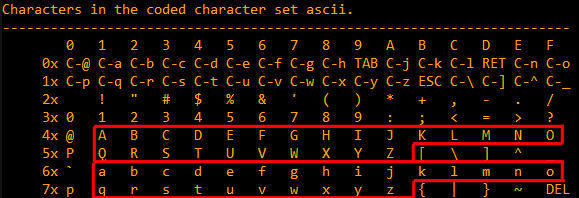
\includegraphics[width=0.7\textwidth]{ascii.png}
\caption{7-битная таблица \ac{ASCII} в Emacs}
\end{figure}

В десятичном виде этот бит это 32 \dots 32?
Но 32 это ASCII-код пробела!

Действительно, можно менять регистр просто применяя XOR к ASCII-коду, с 32 (больше об этом: \myref{toupper_bit}).

Возможно ли, что пустые лакуны в файле это не нулевые байты, а скорее содержащие пробелы?
Еще раз модифицируем наш XOR-ключ (я про-XOR-ю каждый байт ключа с 32):

\begin{lstlisting}[style=custommath]
(* "32" это скаляр, и "key" это вектор, но это OK *)

In[]:= key3 = BitXor[32, key]
Out[]= {112, 86, 34, 84, 81, 70, 86, 57, 67, 40, 51, 55, 84, 93, 75, \
57, 67, 77, 82, 70, 46, 89, 83, 63, 41, 85, 81, 79, 37, 36, 95, 60, \
90, 69, 40, 78, 46, 50, 92, 74, 48, 52, 72, 87, 40, 77, 58, 74, 41, \
65, 45, 67, 47, 87, 52, 73, 85, 66, 71, 86, 33, 94, 61, 65, 90, 49, \
47, 82, 78, 35, 37, 93, 93, 67, 94, 87, 70, 62, 90, 34, 85}

In[]:= DecryptBlock[blk_] := BitXor[key3, blk]
\end{lstlisting}

И снова дешифруем входной файл:

\begin{figure}[H]
\centering
\myincludegraphics{ff/XOR/mask_1/mc_decrypted.png}
\caption{Дешифрованный файл в Midnight Commander, последняя попытка}
\end{figure}

(Расшифрованный файл доступен здесь:
\url{https://github.com/DennisYurichev/RE-for-beginners/blob/master/ff/XOR/mask_1/files/decrypted.dat.bz2}.)

Несомненно, это корректный исходный файл.
Да, и мы видим числа в начале каждого блока. Должно быть это и есть источник некорректного XOR-ключа.
Как выходит, самый встречающийся 81-байтный блок в файле это блок заполненный пробелами и содержащий символ \q{1} на месте
второго байта.
Действительно, как-то так получилось что многие блоки здесь перемежаются с этим блоком.
Может быть это что-то вроде выравнивания (padding) для коротких фраз/сообщений?
Другой часто встречающийся 81-байтный блок также заполнен пробелами, но с другой цифрой, следовательно,
они отличаются только вторым байтом.

Вот и всё! Теперь мы можем написать утилиту для зашифрования файла назад, и, может быть, модифицировать его перед этим

Файл для Mathematica можно скачать здесь:
\url{https://github.com/DennisYurichev/RE-for-beginners/blob/master/ff/XOR/mask_1/files/XOR_mask_1.nb}.

Итог: XOR-шифрование не надежно вообще. Вероятно, разработчик игры хотел просто скрыть внутренности игры от игрока,
ничего более серьезного.
Все же, шифрование вроде этого крайне популярно вследствии его простоты, так что многие реверс инженеры обычно хорошо
с этим знакомы.

